\documentclass[border=1pt]{standalone}
\usepackage[utf8]{luainputenc}
\usepackage[T1]{fontenc}
\usepackage[dvipsnames]{xcolor}
\usepackage{cmbright}
% color list: https://en.wikibooks.org/wiki/LaTeX/Colors

%\definecolor{}{HTML}{}
\definecolor{redplot}{HTML}{D62728}
\definecolor{blueplot}{HTML}{1F77B4}
\definecolor{greenplot}{HTML}{2CA02C}
\definecolor{orangeplot}{HTML}{FF7F0E}

\definecolor{workers}{HTML}{4D8FCB}
\definecolor{evaluators}{HTML}{E8C047}
\definecolor{spectators}{HTML}{D95D5B}
\definecolor{treatment}{HTML}{54B696}

\usepackage{pgfplots}
\pgfplotsset{compat=newest}
\usepgfplotslibrary{units}
\usetikzlibrary{calc}
\usetikzlibrary{patterns,arrows.meta}

%\tikzstyle{greyrectangle} = [rectangle, minimum height=60pt, minimum width=60pt, align=center, draw=gray, fill=gray!7, semithick]

\tikzstyle{cerchiogrigio} = [circle, minimum height=2.6em, align=center, fill=gray!35]

\begin{document}
	
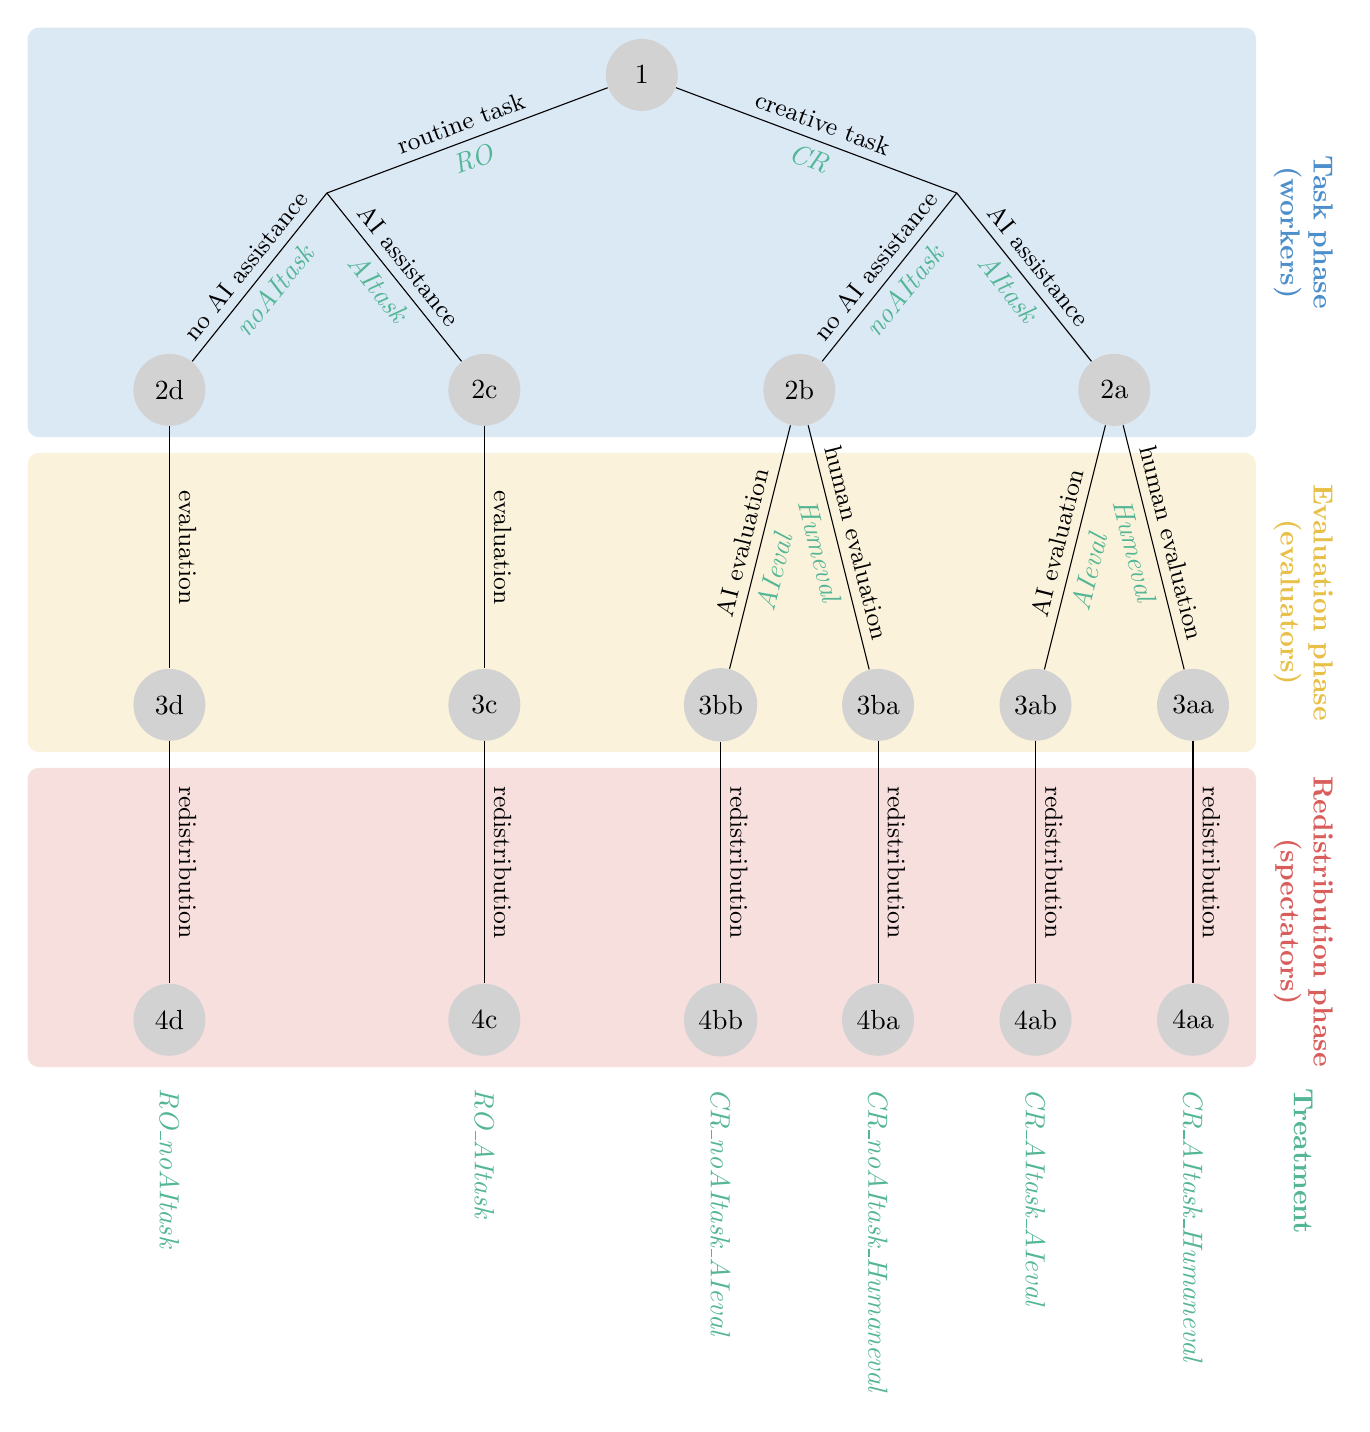
\begin{tikzpicture}[scale=1]
\fill[workers, opacity=.2, rounded corners] (-7.8,7.4) rectangle (7.8,12.6);

\node (1) [cerchiogrigio] at (0,12) {1};
\node (2a) [cerchiogrigio] at (6,8) {2a};
\node (2b) [cerchiogrigio] at (2,8) {2b};
\node (2c) [cerchiogrigio] at (-2,8) {2c};
\node (2d) [cerchiogrigio] at (-6,8) {2d};

\fill[evaluators, opacity=.2, rounded corners] (-7.8,3.4) rectangle (7.8,7.2);
\node (3aa) [cerchiogrigio] at (7,4) {3aa};
\node (3ab) [cerchiogrigio] at (5,4) {3ab};
\node (3ba) [cerchiogrigio] at (3,4) {3ba};
\node (3bb) [cerchiogrigio] at (1,4) {3bb};
\node (3c) [cerchiogrigio] at (-2,4) {3c};
\node (3d) [cerchiogrigio] at (-6,4) {3d};
	
\fill[spectators, opacity=.2, rounded corners] (-7.8,-0.6) rectangle (7.8,3.2);
\node (4aa) [cerchiogrigio] at (7,0) {4aa};
\node (4ab) [cerchiogrigio] at (5,0) {4ab};
\node (4ba) [cerchiogrigio] at (3,0) {4ba};
\node (4bb) [cerchiogrigio] at (1,0) {4bb};
\node (4c) [cerchiogrigio] at (-2,0) {4c};
\node (4d) [cerchiogrigio] at (-6,0) {4d};

\node[rotate=-90, align=center] at (8.4,10) {\color{workers}\textbf{Task phase} \\ \color{workers}\textbf{(workers)}};

\node[rotate=-90, align=center] at (8.4,5.3) {\color{evaluators}\textbf{Evaluation phase} \\ \color{evaluators}\textbf{(evaluators)}};

\node[rotate=-90, align=center] at (8.4,1.25) {\color{spectators}\textbf{Redistribution phase} \\ \color{spectators}\textbf{(spectators)}};



\draw (-4,10.5) --  (1) node[midway, above, sloped, font=\small] {routine task};
\draw[draw=none] (1) -- (-4,10.5)  node[midway, below, sloped] {\color{treatment}\emph{RO}};
\draw (1) -- (4,10.5) node[midway, above, sloped, font=\small] {creative task};
\draw[draw=none] (1) -- (4,10.5) node[midway, below, sloped] {\color{treatment}\emph{CR}};

\draw (-4,10.5) -- (2d) node[midway, above, sloped, font=\small] {no AI assistance};
\draw[draw=none] (-4,10.5) -- (2d) node[midway, below, sloped] {\color{treatment}\emph{noAItask}};
\draw (-4,10.5) -- (2c) node[midway, above, sloped, font=\small] {AI assistance};
\draw[draw=none] (-4,10.5) -- (2c) node[midway, below, sloped] {\color{treatment}\emph{AItask}};

\draw (4,10.5) -- (2a) node[midway, above, sloped, font=\small] {AI assistance};
\draw[draw=none] (4,10.5) -- (2a) node[midway, below, sloped] {\color{treatment}\emph{AItask}};
\draw (4,10.5) -- (2b) node[midway, above, sloped, font=\small] {no AI assistance};
\draw [draw=none] (4,10.5) -- (2b) node[midway, below, sloped] {\color{treatment}\emph{noAItask}};
\draw (2a) -- (3aa) node[midway, above, sloped, font=\small] {human evaluation};
\draw [draw=none] (2a) -- (3aa) node[midway, below, sloped] {\color{treatment}\emph{Humeval}};


\draw (2a) -- (3ab) node[midway, above, sloped, font=\small] {AI evaluation};
\draw [draw=none] (2a) -- (3ab) node[midway, below, sloped, xshift=-7pt] {\color{treatment}\emph{AIeval}};
\draw (2b) -- (3ba) node[midway, above, sloped, font=\small] {human evaluation};
\draw [draw=none] (2b) -- (3ba) node[midway, below, sloped] {\color{treatment}\emph{Humeval}};
\draw (2b) -- (3bb) node[midway, above, sloped, font=\small] {AI evaluation};
\draw[draw=none] (2b) -- (3bb) node[midway, below, sloped, xshift=-7pt] {\color{treatment}\emph{AIeval}};


\draw (2c) -- (3c) node[midway, above, sloped, font=\small] {evaluation};
\draw (2d) -- (3d) node[midway, above, sloped, font=\small] {evaluation};

\draw (3aa) -- (4aa) node[midway, above, sloped, font=\small] {redistribution};
\draw (3ab) -- (4ab) node[midway, above, sloped, font=\small] {redistribution};
\draw (3ba) -- (4ba) node[midway, above, sloped, font=\small] {redistribution};
\draw (3bb) -- (4bb) node[midway, above, sloped, font=\small] {redistribution}; 
\draw (3c) -- (4c) node[midway, above, sloped, font=\small] {redistribution};
\draw (3d) -- (4d) node[midway, above, sloped, font=\small] {redistribution};

\node [anchor=west, rotate=-90] at (8.4,-0.75)  {\color{treatment}\textbf{Treatment}}; %8.4,-0.7

\node [anchor=west, rotate=-90] at (7,-0.75) {\color{treatment}\emph{CR\_AItask\_Humaneval}};
\node [anchor=west, rotate=-90] at (5,-0.75) {\color{treatment}\emph{CR\_AItask\_AIeval}};
\node [anchor=west, rotate=-90] at (3,-0.75) {\color{treatment}\emph{CR\_noAItask\_Humaneval}};
\node [anchor=west, rotate=-90] at (1,-0.75) {\color{treatment}\emph{CR\_noAItask\_AIeval}};
\node [anchor=west, rotate=-90] at (-2,-0.75) {\color{treatment}\emph{RO\_AItask}};
\node [anchor=west, rotate=-90] at (-6,-0.75) {\color{treatment}\emph{RO\_noAItask}};


\end{tikzpicture}
	
\end{document}
